\begin{figure}[!htbp]
    \centering
    
    \begin{tikzpicture}
        [scale=1.2, inner sep=3mm,
        in_node/.style={circle, draw=red!90, fill=red!20,thick,inner sep=0pt, minimum size=3mm},
        out_node/.style={circle, draw=blue!90, fill=blue!20,thick,inner sep=0pt,minimum size=3mm}]
            
        
        %draw model 1st model
        %in nodes
        \node (1stinnode) at (0,0) [in_node] {};
        \node (2ndinnode) at ($(1stinnode)+(0.5,0)$) [in_node] {};
        \node (3rdinnode) at ($(2ndinnode)+(0.5,0)$) [in_node] {};
        %out nodes
        \node (3rdoutnode) at ($(2ndinnode)+(0,1)$) [out_node] {};
        \node (1stoutnode) at ($(3rdoutnode)+(-1,0)$) [out_node] {};
        \node (2ndoutnode) at ($(1stoutnode)+(0.5,0)$) [out_node] {};
        \node (3rdoutnode) at ($(2ndoutnode)+(0.5,0)$) [out_node] {};
        \node (4thoutnode) at ($(3rdoutnode)+(0.5,0)$) [out_node] {};
        \node (5thoutnode) at ($(4thoutnode)+(0.5,0)$) [out_node] {};
        %fully connect nodes
        \draw[->] (1stinnode) -- (1stoutnode);
        \draw[->] (1stinnode) -- (2ndoutnode);
        \draw[->] (1stinnode) -- (3rdoutnode);
        \draw[->] (1stinnode) -- (4thoutnode);
        \draw[->] (1stinnode) -- (5thoutnode);
        \draw[->] (2ndinnode) -- (1stoutnode);
        \draw[->] (2ndinnode) -- (2ndoutnode);
        \draw[->] (2ndinnode) -- (3rdoutnode);
        \draw[->] (2ndinnode) -- (4thoutnode);
        \draw[->] (2ndinnode) -- (5thoutnode);
        \draw[->] (3rdinnode) -- (1stoutnode);
        \draw[->] (3rdinnode) -- (2ndoutnode);
        \draw[->] (3rdinnode) -- (3rdoutnode);
        \draw[->] (3rdinnode) -- (4thoutnode);
        \draw[->] (3rdinnode) -- (5thoutnode);
        %prediction
        %left lower right upper
        \node (1stprediction) at ($(3rdoutnode)+(0,2.8)$) {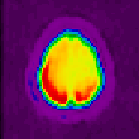
\includegraphics[width=0.17\textwidth]{figures/intro/full_pred.pdf}};
        \draw[->, ultra thick, draw=blue] ($(3rdoutnode)+(0,0.5)$) -- ($(1stprediction)+(0,-1.8)$);
        %x
        \node (input) at ($(2ndinnode)+(0,-2)$) {};
        \node (raw) at ($(input)+(-1.,0)$) {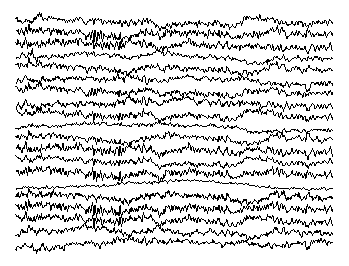
\includegraphics[width=0.08\textwidth]{figures/intro/eeg.pdf}};
        \node (stft) at ($(input)+(1.,0)$) {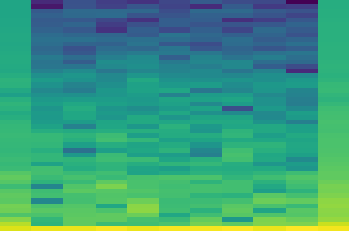
\includegraphics[width=0.09\textwidth]{figures/intro/stft.pdf}};
        \draw[->] ($(raw)+(0.7,0)$) -- ($(stft)+(-0.8,0)$);
        \draw[->, ultra thick, draw=blue] ($(input)+(0,1.1)$) -- ($(2ndinnode)+(0,-0.4)$);

        \node (eeg_legend) at ($(input)+(-3.5,0)$) {};
        \node[align=center] at ($(input)+(-3.7,0)$) {EEG recording\\Time frequency\\STFT domain};
        \node (model_legend) at ($(2ndinnode)+(-3.5,0.5)$) {Model};
        \node (fmri_legend) at ($(1stprediction)+(-3.5,0)$) {fMRI prediction};
        %table like lines
        \draw[dotted, opacity=0.8] ($(eeg_legend)+(-2,1.3)$) -- ($(eeg_legend)+(11.8,1.3)$);
        \draw[dotted, opacity=0.8] ($(model_legend)+(-2,1.15)$) -- ($(model_legend)+(11.8,1.15)$);

        
        
        %draw model 2nd 
        %in nodes
        \node (1stinnode) at ($(1stinnode)+(6.5,0)$) [in_node] {};
        \node (2ndinnode) at ($(1stinnode)+(0.5,0)$) [in_node] {};
        \node (3rdinnode) at ($(2ndinnode)+(0.5,0)$) [in_node] {};
        %out nodes
        \node (2ndoutnode) at ($(2ndinnode)+(0,1)$) [out_node] {};
        \node (3rdoutnode) at ($(2ndoutnode)+(0.5,0)$) [out_node] {};
        \node (1stoutnode) at ($(3rdoutnode)+(-1,0)$) [out_node] {};
        %fully connect nodes
        \draw[->] (1stinnode) -- (1stoutnode);
        \draw[->] (1stinnode) -- (2ndoutnode);
        \draw[->] (1stinnode) -- (3rdoutnode);
        \draw[->] (2ndinnode) -- (1stoutnode);
        \draw[->] (2ndinnode) -- (2ndoutnode);
        \draw[->] (2ndinnode) -- (3rdoutnode);
        \draw[->] (3rdinnode) -- (1stoutnode);
        \draw[->] (3rdinnode) -- (2ndoutnode);
        \draw[->] (3rdinnode) -- (3rdoutnode);
        %prediction
        \node (2ndprediction) at ($(2ndoutnode)+(0,2.8)$) {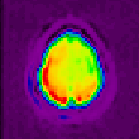
\includegraphics[width=0.17\textwidth]{figures/intro/relaxed_pred.pdf}};
        \draw[->, ultra thick, draw=blue] ($(2ndoutnode)+(0,0.5)$) -- ($(2ndprediction)+(0,-1.8)$);
        %eeg x
        \node (input) at ($(2ndinnode)+(0,-2)$) {};
        \node (raw) at ($(input)+(-1.,0)$) {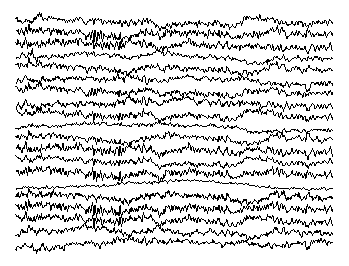
\includegraphics[width=0.08\textwidth]{figures/intro/eeg.pdf}};
        \node (stft) at ($(input)+(1.,0)$) {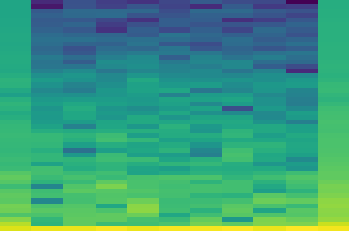
\includegraphics[width=0.09\textwidth]{figures/intro/stft.pdf}};
        \draw[->] ($(raw)+(0.7,0)$) -- ($(stft)+(-0.8,0)$);
        \draw[->, ultra thick, draw=blue] ($(input)+(0,1.1)$) -- ($(2ndinnode)+(0,-0.4)$);
        %problem relaxation
        \draw[->, ultra thick] ($(5thoutnode)+(0.5,0.5)$) -- ($(1stoutnode)+(-0.5,0.5)$);
        \node[align=center] (description) at ($(5thoutnode)+(2.45,-0.5)$) {predict less\\features};

        \node at ($(fmri_legend)+(0,2.1)$) {Resolution};
        \node at ($(1stprediction)+(0,2.1)$) {full};
        \node at ($(2ndprediction)+(0,2.1)$) {lower};
        \draw[opacity=0.4] ($(fmri_legend)+(-2,1.7)$) -- ($(fmri_legend)+(11.8,1.7)$);

        \node at ($(1stprediction)+(2.3,0.8)$) {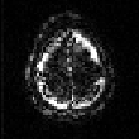
\includegraphics[width=0.065\textwidth]{figures/intro/full_res.pdf}};
        \node at ($(2ndprediction)+(-2.3,0.8)$) {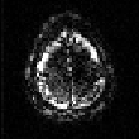
\includegraphics[width=0.065\textwidth]{figures/intro/relaxed_res.pdf}};
        
    \end{tikzpicture}
    \caption{EEG-to-fMRI synthesis and the spectral relaxation. EEG windows are transformed to the time--frequency (STFT) domain and mapped to an fMRI volume. The relaxed decoder predicts only the low spatial frequencies of the volume (fewer outputs, right) instead of the full resolution (left), consistent with the low spatial resolution of the EEG. The predictions are real outputs for a CHUR-XP2 test subject (axial slice 20): the stochastic spectral decoder, whose samples span the full resolution (left), and the zero-filled heteroscedastic network (right); the small grey maps beside them are their absolute residues; we also quantify what such a relaxed decoder can and cannot express.}
    \label{fig:idea_description}
\end{figure}
